\section{识别结果分析}

采用交叉验证的方法来评价分类器的性能好坏,所选用的数据集中的类别如图~\ref{fig: ratio}所示,其中有10个是浮游动物类,包括Appendicularia(被囊类)、Chaetognatha(毛颚类)、CladoceraPenilia(枝角类喙)、Copepoda(桡足类)、Decapoda(十足类)、Doliolida(海樽类)、Egg(蛋类)、Pteropoda(翼足类)、Gelatinous(凝胶纤维)、Multiple。3个非浮游动物类:Nonbio(非生物类)、Bubble(气泡)、Fiber(纤维)。将该数据集随机均分为$n$份,其中每个子集数据分别做一次验证集,其余的$n-1$组子集数据作为训练集,这样会得到$n$个模型,用这$n$个模型最终的验证集的分类准确率的平均数作为此分类器的性能指标。

采用随机森林学习算法,67个特征的评价结果如图~\ref{fig: RandomForest}。

\begin{figure}[!ht]
\centering
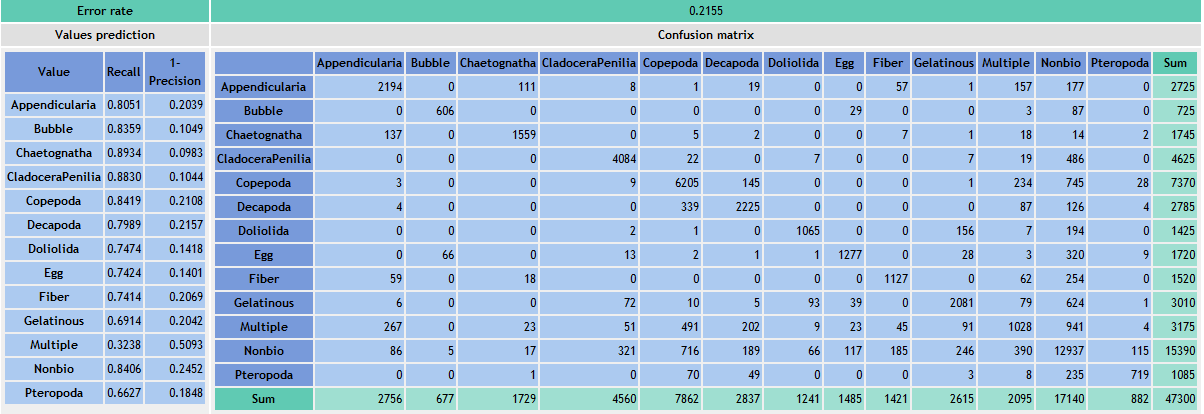
\includegraphics[width=1.0\textwidth]{RandomForest.png}
\caption{Random Forest}
\label{fig: RandomForest}
\end{figure} 

采用随机森林算法,去掉以下位置特征(XM, YM, BX, BY, Width, Height, Angle, XStart, YStart, XMg5, YMg5, X, Y)的评价结果如图~\ref{fig: withoutposition},可以看到,与用所有特征相比,去除不必要的位置特征会使评价结果有所提高,对所有种类的Recall值、Precision值求平均(除了Multi类),得到的平均的Recall值为0.799,平均的Precision值为0.161。PID文件中的位置特征大多是ImageJ自带的,是用来生成缩略图所需的参数,在训练分类器时并没有使用。

\begin{figure}[!ht]
\centering
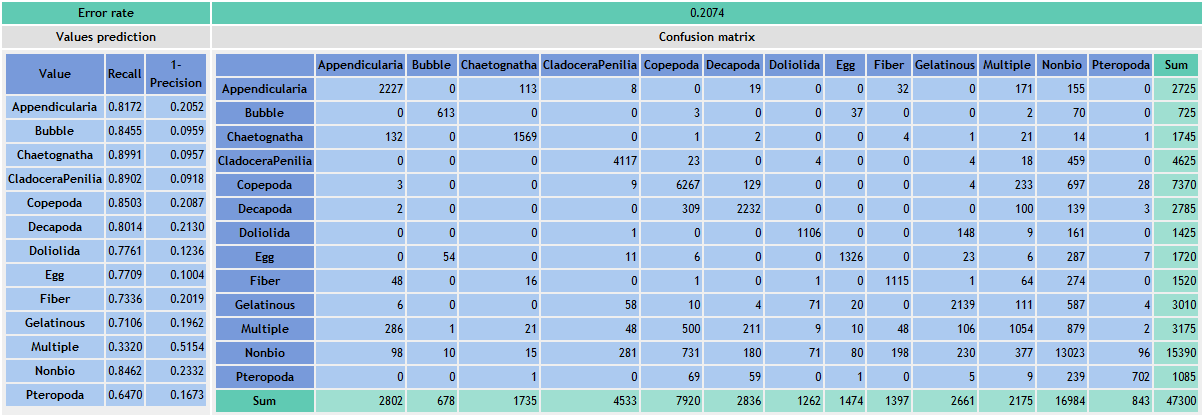
\includegraphics[width=1.0\textwidth]{withoutposition.png}
\caption{Random Forest (without position variables)}
\label{fig: withoutposition}
\end{figure} 

采用K-NN算法,去掉位置特征后的评价结果如图~\ref{fig: KNN}。

\begin{figure}[!ht]
\centering
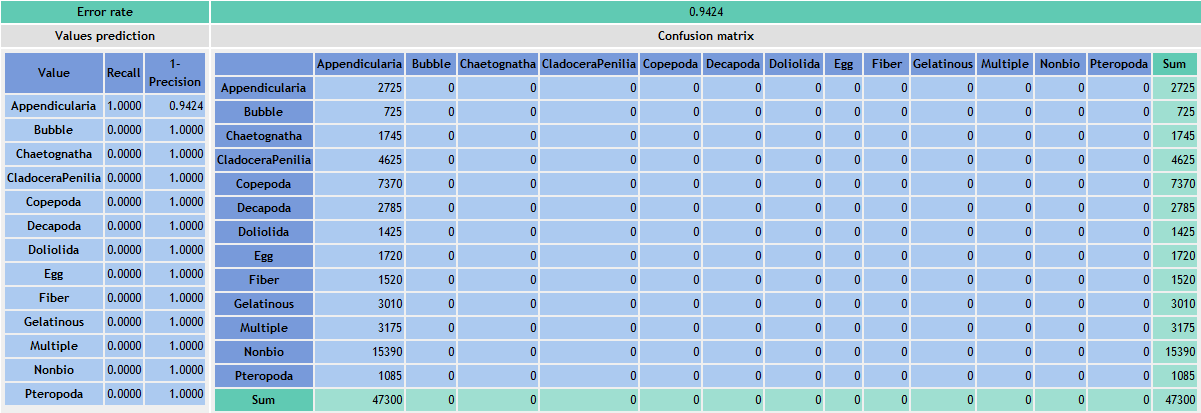
\includegraphics[width=1.0\textwidth]{KNN.png}
\caption{K-NN (without position variables)}
\label{fig: KNN}
\end{figure} 

采用C-SVC linear算法,去掉位置特征后的评价结果如图~\ref{fig: C-SVClinear}。

\begin{figure}[!ht]
\centering
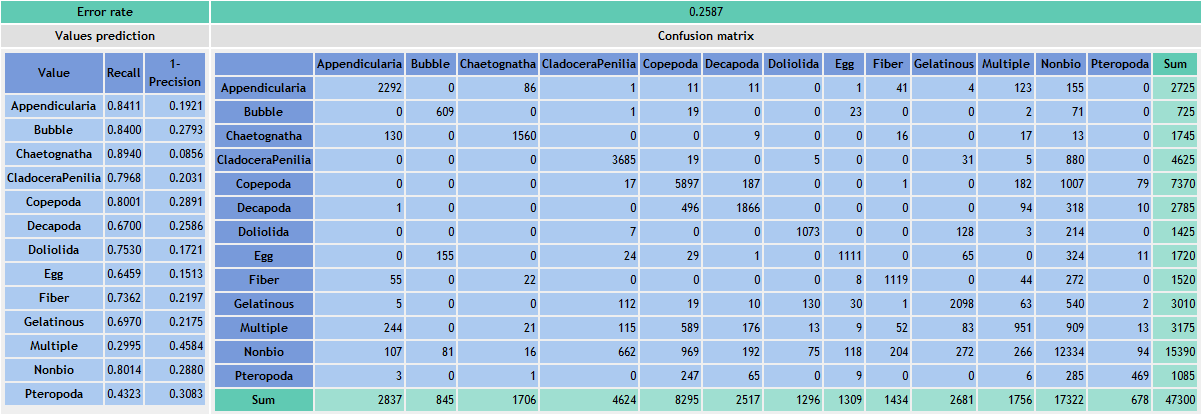
\includegraphics[width=1.0\textwidth]{C-SVClinear.png}
\caption{C-SVC linear (without position variables)}
\label{fig: C-SVClinear}
\end{figure} 

采用C-SVC RBF算法,去掉位置特征后的评价结果如图~\ref{fig: C-SVC-RBF}。

\begin{figure}[!ht]
\centering
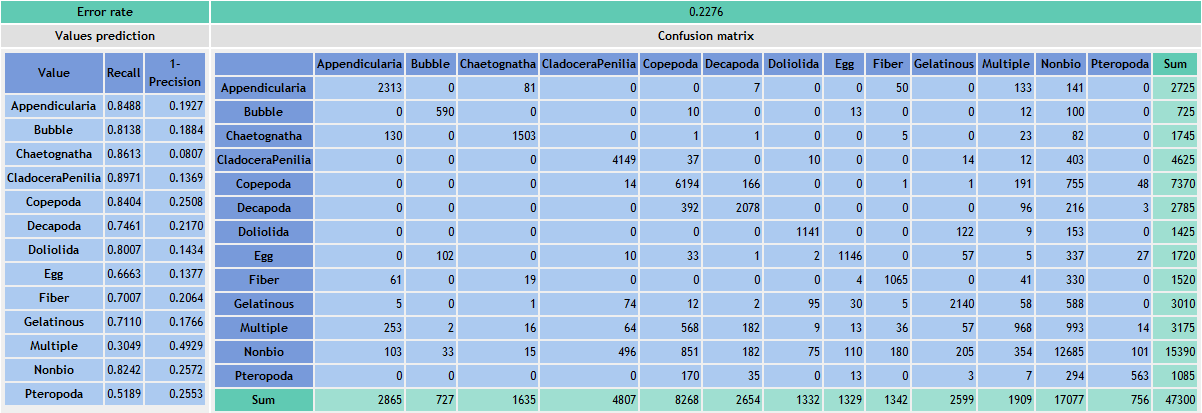
\includegraphics[width=1.0\textwidth]{C-SVC-RBF.png}
\caption{C-SVC RBF (without position variables)}
\label{fig: C-SVC-RBF}
\end{figure} 

采用BVM RBF算法,去掉位置特征后的评价结果如图~\ref{fig: BVM-RBF}。

\begin{figure}[!ht]
\centering
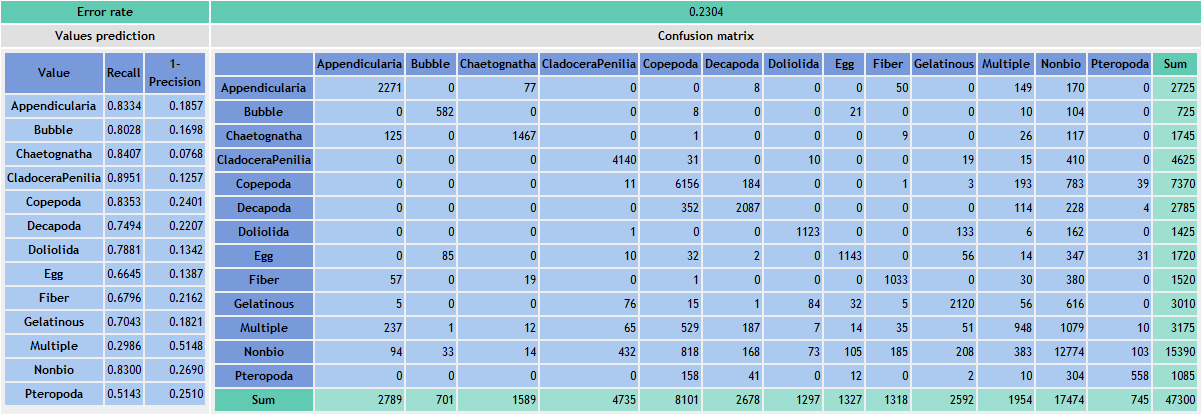
\includegraphics[width=1.0\textwidth]{BVM-RBF.png}
\caption{BVM RBF (without position variables)}
\label{fig: BVM-RBF}
\end{figure} 

采用PLS算法,去掉位置特征后的评价结果如图~\ref{fig: PLS}。

\begin{figure}[!ht]
\centering
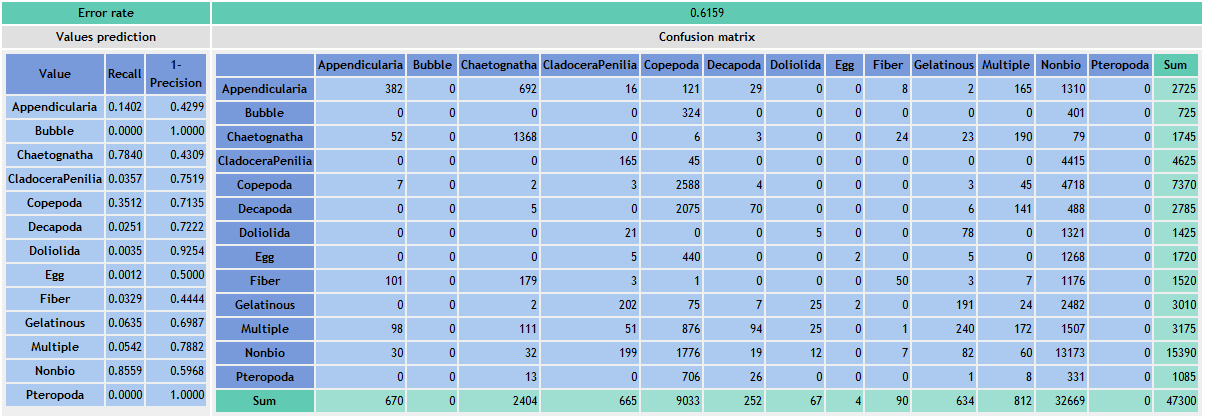
\includegraphics[width=1.0\textwidth]{PLS.png}
\caption{PLS (without position variables)}
\label{fig: PLS}
\end{figure} 

采用Multilayer perceptron算法,去掉位置特征后的评价结果如图~\ref{fig: MultilayerPerceptron}。

\begin{figure}[!ht]
\centering
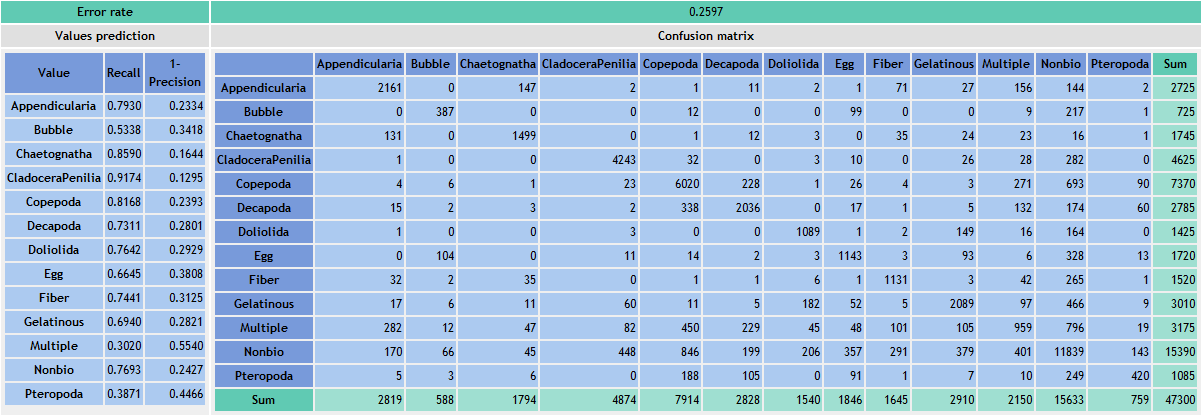
\includegraphics[width=1.0\textwidth]{MultilayerPerceptron.png}
\caption{MultilayerPerceptron (without position variables)}
\label{fig: MultilayerPerceptron}
\end{figure} 

\section{优缺点分析}

PkID主要用了灰度特征、尺寸特征和形状特征。其中灰度特征跟灰度图的质量有很大关系,并不能完全准确地将不同种类区分开来,这里可以尝试加入一些灰度对比度特征。对于尺寸特征,每幅图像中都有一个5mm的标尺,可以依据标尺来度量物体的一些长度特征。人在进行浮游动物分类时,主要是依据形状特征,所以形状特征应该是最重要的,但PkID中只采用了少数简单的形状特征,因而不能充分地表示某一类浮游动物。

对于具体哪些特征是有用的哪些是没用的,还得通过具体的实验才能看出来。单从缩略图来看,这三类特征都是有用的,都有区分作用,但是还不充足,还应该再加入一些更合理的特征。
